\documentclass[tikz,border=3pt]{standalone}
\usepackage[utf8]{inputenc}
\usepackage[T1]{fontenc}
\usepackage{lmodern}
\renewcommand{\familydefault}{\sfdefault}
\usepackage{sansmath}\sansmath
\usepackage{chemfig}
\usepackage{pgfplots}\pgfplotsset{compat=1.18,/pgf/number format/use comma,/pgf/number format/1000 sep={.}}
\usetikzlibrary{arrows.meta,calc,positioning,decorations.pathmorphing,patterns}
% paleta del sitio
\definecolor{nar}{HTML}{E8680C}\definecolor{narc}{HTML}{FFB35C}\definecolor{hielo}{HTML}{FFF3E8}
\definecolor{tinta}{HTML}{1D1D1F}\definecolor{gris}{HTML}{6E6E73}\definecolor{lila}{HTML}{7C5CF0}
\definecolor{azul}{HTML}{2F6FD6}\definecolor{menta}{HTML}{17A673}\definecolor{coral}{HTML}{E8342A}
\begin{document}
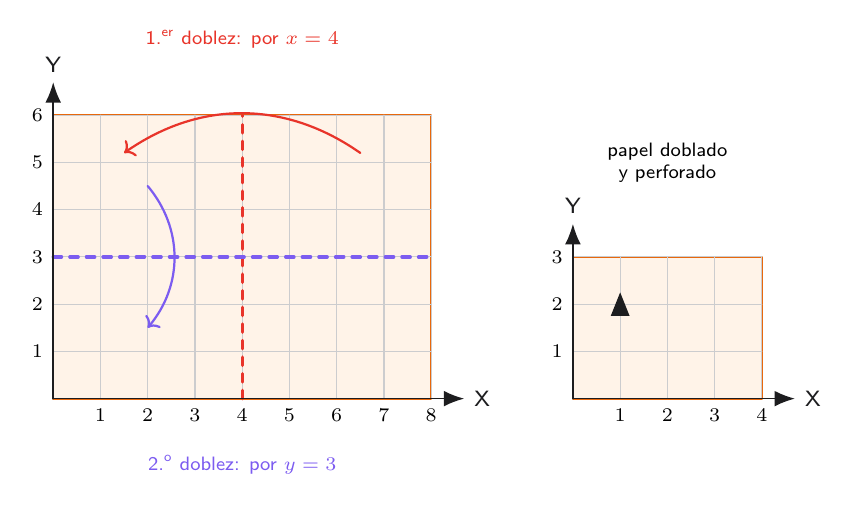
\begin{tikzpicture}[font=\small,x=0.6cm,y=0.6cm,line cap=round,line join=round,step={(1,1)}]
\filldraw[fill=hielo,draw=nar,thick] (0,0) rectangle (8,6);
\draw[gris!35,thin] (0,0) grid (8,6);
\draw[coral,very thick,dashed] (4,0)--(4,6); \draw[lila,very thick,dashed] (0,3)--(8,3);
\node[font=\scriptsize,text=coral,inner sep=1pt] at (4,7.6) {1.\textsuperscript{er} doblez: por $x = 4$};
\node[font=\scriptsize,text=lila,inner sep=1pt] at (4,-1.4) {2.\textsuperscript{o} doblez: por $y = 3$};
\draw[->,coral,thick] (6.5,5.2) to[bend right=35] (1.5,5.2);
\draw[->,lila,thick] (2,4.5) to[bend left=40] (2,1.5);
\draw[-{Latex[length=2.6mm,width=2mm]},tinta,semithick] (0,0)--(8.7,0) node[right,font=\footnotesize] {X};
\draw[-{Latex[length=2.6mm,width=2mm]},tinta,semithick] (0,0)--(0,6.7) node[above,font=\footnotesize] {Y};
\node[below,font=\scriptsize,inner sep=1.5pt,fill=white,fill opacity=.85,text opacity=1] at (1,-0.12) {$1$};
\node[below,font=\scriptsize,inner sep=1.5pt,fill=white,fill opacity=.85,text opacity=1] at (2,-0.12) {$2$};
\node[below,font=\scriptsize,inner sep=1.5pt,fill=white,fill opacity=.85,text opacity=1] at (3,-0.12) {$3$};
\node[below,font=\scriptsize,inner sep=1.5pt,fill=white,fill opacity=.85,text opacity=1] at (4,-0.12) {$4$};
\node[below,font=\scriptsize,inner sep=1.5pt,fill=white,fill opacity=.85,text opacity=1] at (5,-0.12) {$5$};
\node[below,font=\scriptsize,inner sep=1.5pt,fill=white,fill opacity=.85,text opacity=1] at (6,-0.12) {$6$};
\node[below,font=\scriptsize,inner sep=1.5pt,fill=white,fill opacity=.85,text opacity=1] at (7,-0.12) {$7$};
\node[below,font=\scriptsize,inner sep=1.5pt,fill=white,fill opacity=.85,text opacity=1] at (8,-0.12) {$8$};
\node[left,font=\scriptsize,inner sep=1.5pt,fill=white,fill opacity=.85,text opacity=1] at (-0.12,1) {$1$};
\node[left,font=\scriptsize,inner sep=1.5pt,fill=white,fill opacity=.85,text opacity=1] at (-0.12,2) {$2$};
\node[left,font=\scriptsize,inner sep=1.5pt,fill=white,fill opacity=.85,text opacity=1] at (-0.12,3) {$3$};
\node[left,font=\scriptsize,inner sep=1.5pt,fill=white,fill opacity=.85,text opacity=1] at (-0.12,4) {$4$};
\node[left,font=\scriptsize,inner sep=1.5pt,fill=white,fill opacity=.85,text opacity=1] at (-0.12,5) {$5$};
\node[left,font=\scriptsize,inner sep=1.5pt,fill=white,fill opacity=.85,text opacity=1] at (-0.12,6) {$6$};
\begin{scope}[xshift=6.6cm]
\filldraw[fill=hielo,draw=nar,thick] (0,0) rectangle (4,3); \draw[gris!35,thin] (0,0) grid (4,3);
\fill[tinta] (0.8,1.75)--(1.2,1.75)--(1,2.25)--cycle;
\draw[-{Latex[length=2.6mm,width=2mm]},tinta,semithick] (0,0)--(4.7,0) node[right,font=\footnotesize] {X};
\draw[-{Latex[length=2.6mm,width=2mm]},tinta,semithick] (0,0)--(0,3.7) node[above,font=\footnotesize] {Y};
\node[below,font=\scriptsize,inner sep=1.5pt,fill=white,fill opacity=.85,text opacity=1] at (1,-0.12) {$1$};
\node[below,font=\scriptsize,inner sep=1.5pt,fill=white,fill opacity=.85,text opacity=1] at (2,-0.12) {$2$};
\node[below,font=\scriptsize,inner sep=1.5pt,fill=white,fill opacity=.85,text opacity=1] at (3,-0.12) {$3$};
\node[below,font=\scriptsize,inner sep=1.5pt,fill=white,fill opacity=.85,text opacity=1] at (4,-0.12) {$4$};
\node[left,font=\scriptsize,inner sep=1.5pt,fill=white,fill opacity=.85,text opacity=1] at (-0.12,1) {$1$};
\node[left,font=\scriptsize,inner sep=1.5pt,fill=white,fill opacity=.85,text opacity=1] at (-0.12,2) {$2$};
\node[left,font=\scriptsize,inner sep=1.5pt,fill=white,fill opacity=.85,text opacity=1] at (-0.12,3) {$3$};
\node[font=\scriptsize,align=center] at (2,5.0) {papel doblado\\y perforado};
\end{scope}
\end{tikzpicture}
\end{document}
